%%%%%%%%%%%%%%%%%%%%%%%%%%%%%%%%%%%%% 
%% LE2I beamer template
%% Guillaume Lemaitre, October 2014
%%%%%%%%%%%%%%%%%%%%%%%%%%%%%%%%%%%%% 

\documentclass{beamer}

\usepackage[utf8]{inputenc}
\usepackage[T1]{fontenc} 
\usetheme{le2i} 

%% The amssymb package provides various useful mathematical symbols
\usepackage{amssymb}
%% The amsthm package provides extended theorem environments
\usepackage{amsthm}
%% amsmath for math environment
\usepackage{amsmath}

\DeclareMathOperator*{\argmin}{arg\,min}
\DeclareMathOperator*{\argmax}{arg\,max}
\DeclareMathOperator*{\sign}{sign}

\usepackage{booktabs}
\usepackage{siunitx}

%% figure package
\usepackage{epsf,graphicx}
\usepackage{epstopdf}
\usepackage{subfig}
\usepackage{transparent}

%% In order to draw some graphs
\usepackage{tikz,xifthen}
\usepackage{tikz-qtree}
\usepackage{adjustbox}
\usetikzlibrary{decorations.pathmorphing}
\usetikzlibrary{fit}
\usetikzlibrary{backgrounds}
\usetikzlibrary{shapes,arrows,shadows}
\usetikzlibrary{calc,decorations.pathreplacing,decorations.markings,positioning}
\usetikzlibrary{snakes,decorations.text,shapes,patterns}
% \usepackage{scalefnt,lmodern,booktabs}

%% Package for cross and tick symbols
\usepackage{pifont}
\newcommand{\tick}{\color{green!60!black!80}\ding{51}}
\newcommand{\cross}{\color{red!60!black!80}\ding{55}}

\title{\large Estimating Power without Measuring it: \small a Machine Learning Approach}
\author{\textit{Guillaume Lema\^itre} \& C\'edric Lema\^itre \\ \ \\ \tiny
  \texttt{guillaume.lemaitre@inria.fr} \\ \texttt{contact@apeira-technologies.fr} \\ \ }
\date{Science \& Cycling \\ 4\textsuperscript{th} July 2018}

\institute{Inria --- Paris-Saclay Center for Data Science \\ Apeira Technologies}

%% Uncomment if you want to avoid thousand of bullet inside the menu
% \usepackage{etoolbox}
% \makeatletter
% \patchcmd{\slideentry}{\advance\beamer@xpos by1\relax}{}{}{}
% \def\beamer@subsectionentry#1#2#3#4#5{\advance\beamer@xpos by1\relax}%
% \makeatother

\begin{document}

% Show the title page
\begin{frame}
  \titlepage
\end{frame}

% Show the table of contents
\begin{frame}
  \tableofcontents[sectionstyle=show,subsectionstyle=show,subsubsectionstyle=hide]
\end{frame}

% \section{First section}

% \subsection{First subsection}

% \begin{frame}
%   \frametitle{A Kick-Ass Title}
%   \framesubtitle{A Kick-Ass Title Subtitle}
%   \begin{block}{Block environment}
%     \begin{itemize}
%     \item Item 1
%     \item Item 2
%     \end{itemize}
%   \end{block}
%   \begin{figure}
%     \centering
%     
\includegraphics[width=.2\textwidth]{./images/logos/le2i-logo.pdf}
%     \caption{Include an image}
%   \end{figure}
% \end{frame}

% \subsection{Second subsection}

% \begin{frame}
%   \frametitle{A Kick-Ass Title}
%   \framesubtitle{A Kick-Ass Title Subtitle}
%   \begin{block}{Block environment}
%     \begin{itemize}
%     \item[\cross] Cross item
%     \item[\tick] Tick item
%     \end{itemize}
%   \end{block}
%   \begin{equation}
%     \label{eq:eq1}
%     f(x)=ax+b \ .
%   \end{equation}
% \end{frame}


\section{Introduction}

\subsection{Context}

\begin{frame}
  \frametitle{Introduction}
  \framesubtitle{Context}
  \begin{block}{\small Problematic}\centering
    Estimate power from heterogeneous data sensor
  \end{block}
  \begin{block}{\small Saris PowerTap PowerCal}
    \begin{itemize}\small
    \item Low-cost power-meter based on heart-rate
    \item[\tick] Low-cost device
    \item[\cross] Not suitable to track small power changes
    \end{itemize}
  \end{block}
  \begin{block}{\small Strava}
    \begin{itemize}\small
    \item Large amount of data
    \item Mathematical model based on mechanic
    \end{itemize}
  \end{block}
  % \begin{equation}
  %   \label{eq:eq1}
  %   f(x)=ax+b \ .
  % \end{equation}
\end{frame}

\subsection{State-of-the-art}

\begin{frame}
  \frametitle{Introduction}
  \framesubtitle{State-of-the-art}
  \begin{block}{\small Mathematical model based on mechanic}
    \begin{equation}
      \small
      \label{eq:eq1}
      P_{meca} = \left( 0.5 \rho S C_{x} V_{a}^{2} + C_{r} m g \cos \alpha + m g \sin
        \alpha \right) V_{d} \ .
    \end{equation}
  \end{block}
  \begin{block}{\small Model parameters}
    \begin{table}
      \centering
      \scriptsize
      \begin{tabular}{lcc}
        \toprule
        \textbf{Name} & \textbf{Symbol} & \textbf{Unit} \\
        \midrule
        Air density & $\rho$ & \si{\kilo\gram\per\cubic\meter} \\
        Frontal surface & $S$ & \si{\meter\squared} \\
        Drag coefficient & $C_{x}$ & NA\\
        Air speed & $V_{a}$ & \si{\meter\per\second} \\
        Rolling coefficient & $C_{r}$ & NA \\
        Mass of rider and bike & $m$ & \si{\kilo\gram} \\
        Gravitational constant & $g$ & \si{\meter\per\second\squared} \\
        Slope & $\alpha$ & \si{\radian} \\
        Rider speed & $V_{d}$ & \si{\meter\per\second} \\
        \bottomrule
      \end{tabular}
    \end{table}
  \end{block}
\end{frame}


\section{Methods}

\begin{frame}
  \frametitle{Power estimation using machine learning}
  \framesubtitle{\ }
  \begin{figure}
    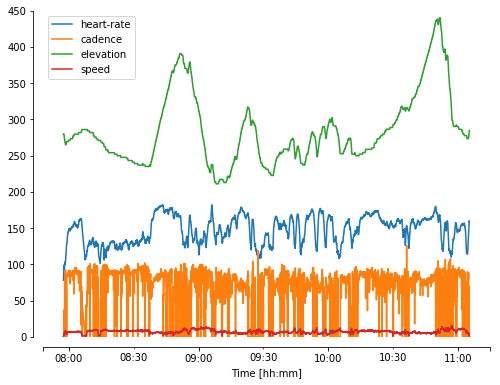
\includegraphics[width=.7\textwidth]{./images/original_data.png}
    \caption{Original data}
  \end{figure}
\end{frame}

\begin{frame}
  \frametitle{Power estimation using machine learning}
  \framesubtitle{\ }
  \begin{block}{Feature engineering}
    \begin{itemize}
    \item Compute gradient for some data (acceleration, elevation, heart-rate)
    \item Compute derivative with different time periods (\SI{1}{\second} ---
      \SI{5}{\second})
    \item Total of 48 features
    \end{itemize}
  \end{block}
  \begin{block}{Regressor}
    \begin{itemize}
    \item Gradient boosting machine
    \end{itemize}
  \end{block}
\end{frame}

\section{Experiments}

\subsection{Materials}

\begin{frame}
  \frametitle{Experiments}
  \framesubtitle{Setup}
  \begin{block}{\small Data set}
    \begin{itemize}\small
    \item 5 riders
    \item 4 power meters: Saris PowerTap, Rotor Power LT, Power2Max, and SRM
    \item 417 rides
    \end{itemize}
  \end{block}
  \begin{block}{\small Model validation}
    \begin{itemize}\small
    \item Group $k$-fold cross-validation with $k=3$
    \end{itemize}
  \end{block}
  \begin{block}{\small Model evaluation}
    \begin{itemize}\small
    \item Coefficient of determination R$^2$
    \item Median absolute error (MAE)
    \end{itemize}
  \end{block}
\end{frame}

\subsection{Hyper-parameters}

\begin{frame}
  \frametitle{Experiments}
  \framesubtitle{Model hyper-parameters}
  \begin{columns}
    \begin{column}{0.5\textwidth}
      \begin{block}{\small Mathematical model}
        \begin{table}
          \centering
          \scriptsize
          \begin{tabular}{lr}
            \toprule
            \textbf{Parameter} & \textbf{Value} \\
            \midrule
            Rider weight & Specific \\
            Bike weight & \SI{6.8}{\kilo\gram} \\
            Rolling coefficient $C_{r}$ & 0.0045 \\
            Atmospheric pressure & \SI{1013}{\hecto\pascal} \\
            $S C_{x}$ & \SI{0.32}{\meter\squared} \\
            Temperature & \SI{15}{\celsius} \\
            \bottomrule
          \end{tabular}
        \end{table}
      \end{block}
    \end{column}
    \begin{column}{0.5\textwidth}  %%<--- here
      \begin{block}{\small Machine learning model}
        \begin{table}
          \centering
          \scriptsize
          \begin{tabular}{lr}
            \toprule
            \textbf{Parameter} & \textbf{Value} \\
            \midrule
            Number of decision tree & 200 \\
            Depth of each decision tree & 8 \\
            \bottomrule
          \end{tabular}
        \end{table}
      \end{block}
    \end{column}
  \end{columns}
\end{frame}

\section{Results}

\subsection{Performance}

\begin{frame}
  \frametitle{Results}
  \framesubtitle{Quantitative results}
  \begin{columns}
    \begin{column}{0.5\textwidth}
      \begin{block}{\small R$^2$ and MAE scores}
        \begin{table}
          \scriptsize
          \centering
          \begin{tabular}{lcc}
            \toprule
            \textbf{Metric} & \textbf{Math} & \textbf{ML} \\
            \midrule
            R$^2$ & -0.55 & 0.76 \\
            MAE & 61.09 & 21.95 \\
            \bottomrule
          \end{tabular}
        \end{table}
      \end{block}
    \end{column}
    \begin{column}{0.5\textwidth}  %%<--- here
      \begin{figure}
        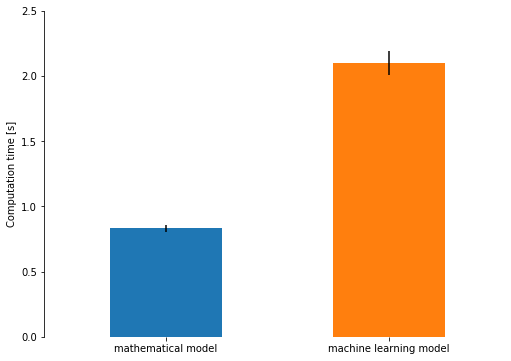
\includegraphics[width=1.0\textwidth]{./images/scoring_time.png}
        \caption{Computation time for estimation around 1 million samples}
      \end{figure}
    \end{column}
  \end{columns}
\end{frame}

\subsection{Zoom-in}

\begin{frame}
  \frametitle{Results}
  \framesubtitle{Zoom-in}
  \begin{figure}
    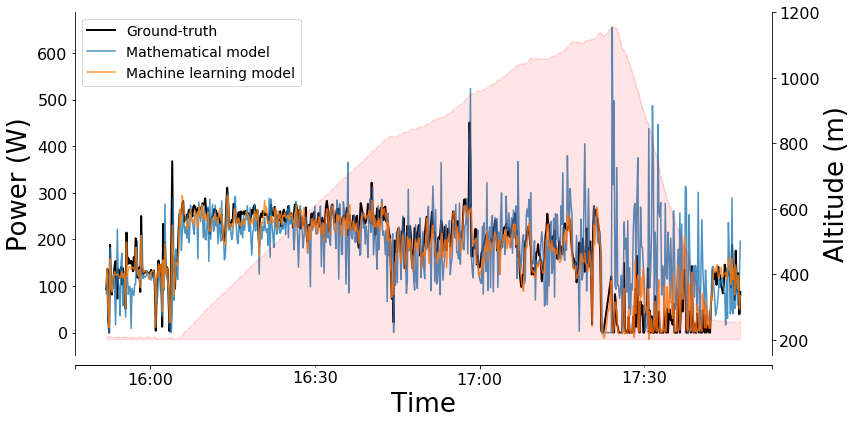
\includegraphics[width=.95\textwidth]{./images/uphill-downhill-profile.png}
    \caption{Power estimation for uphill and downhill}
  \end{figure}
\end{frame}

\begin{frame}
  \frametitle{Results}
  \framesubtitle{Zoom-in}
  \begin{figure}
    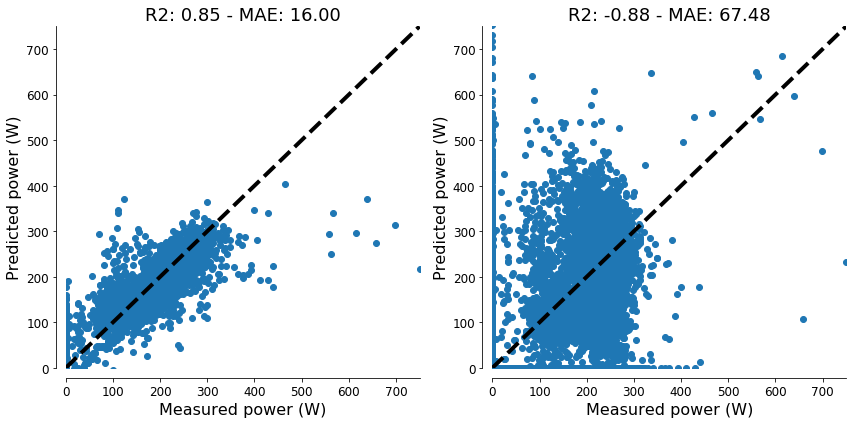
\includegraphics[width=.95\textwidth]{./images/uphill-downhill-r2.png}
    \caption{Left: Machine learning model --- right: mathematical model}
  \end{figure}
\end{frame}

\begin{frame}
  \frametitle{Results}
  \framesubtitle{Zoom-in}
  \begin{figure}
    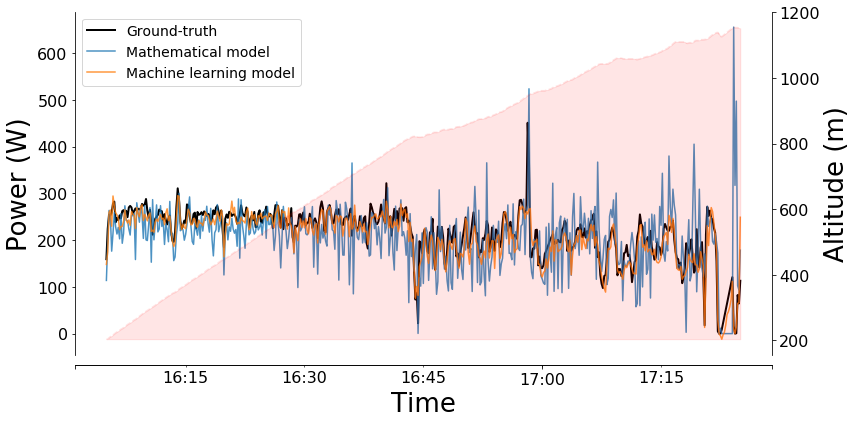
\includegraphics[width=.95\textwidth]{./images/uphill-profile.png}
    \caption{Power estimation for uphill}
  \end{figure}
\end{frame}

\begin{frame}
  \frametitle{Results}
  \framesubtitle{Zoom-in}
  \begin{figure}
    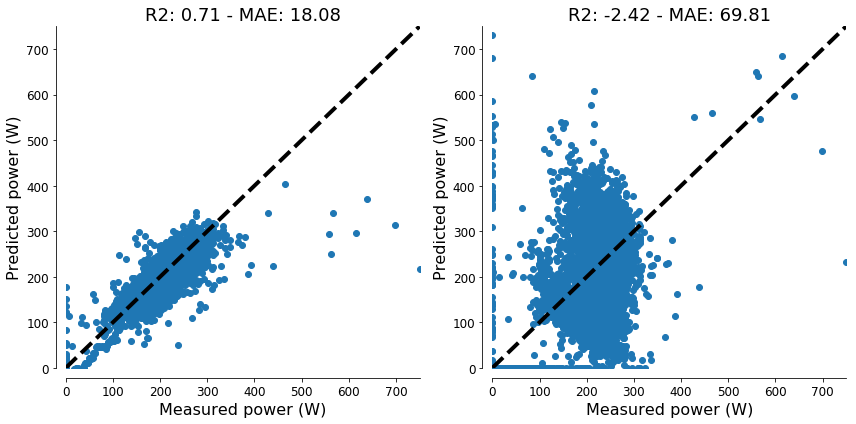
\includegraphics[width=.95\textwidth]{./images/uphill-r2.png}
    \caption{Left: Machine learning model --- right: mathematical model}
  \end{figure}
\end{frame}

\subsection{Summary}

\begin{frame}
  \frametitle{Results}
  \framesubtitle{Summary}
  \begin{block}{\small Mathematical model}
    \begin{itemize}\small
    \item[\tick] Fast prediction
    \item[\cross] Too much unknown parameters
    \item[\cross] Too much variation in the estimation
    \end{itemize}
  \end{block}
  \begin{block}{\small Machine learning model}
    \begin{itemize}\small
    \item[\tick] Fast prediction
    \item[\tick] Better prediction 
    \item[\cross] Difficulty to predict short power peak
    \end{itemize}
  \end{block}
\end{frame}

\subsection{Post-analysis}

\begin{frame}
  \frametitle{Results}
  \framesubtitle{Analysis of the machine learning model}
  \begin{figure}
    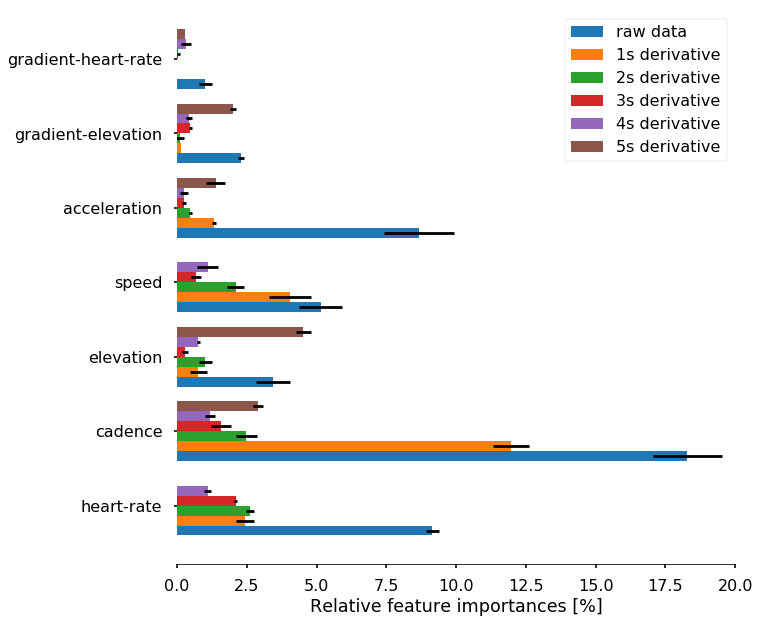
\includegraphics[width=.7\textwidth]{./images/feature_importances.png}
    \caption{Feature importances of the different features used in the model}
  \end{figure}
\end{frame}

\section{Future work}

\begin{frame}
  \frametitle{Future work}
  \framesubtitle{\ }
  \begin{block}{\small Extension of the current work}
    \begin{itemize}\small
    \item[\tick] Convolutional neural-network
    \item[\cross] Larger data set
    \end{itemize}
  \end{block}
  \begin{block}{\small Open-source initiative via GoldenCheetah}
    \begin{itemize}\small
    \item OpenData collection
    \item Development of \texttt{scikit-sports}
    \end{itemize}
  \end{block}
  \begin{block}{\small Purpose}
    \begin{itemize}\small
    \item[\tick] Reproducibility of analysis and methods
    \item[\tick] Use data science tools to solve different problematic in
      cycling performance 
    \end{itemize}
  \end{block}
\end{frame}

\end{document}
